\section{LSTM Method}
The lstm...

% Train val split
When working with time series it is important to think about how one splits up
the dataset into training, validation, and test set.
One key aspect when forecasting a time series is the newer the information,
the more relevant it is for the forecast.
In a perfect world the model will be able to use all the available data for training,
right up to the point of forecast, then try to forecast the wanted horizon.
However, in order to tune hyperparameters and avoid overfitting to the training
set, we need a validation set.
In a stateful LSTM everything fed through the network is seen by the network
as follow each other in time. Since the validation step is executed at the end of
each epoch, and each epoch pass feeds all the training data through the network,
it makes sense to use the last section of the training data as the validation data.

\begin{figure}[h!]
  \centering
  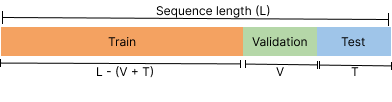
\includegraphics[width=0.7\textwidth]{./figs/illustrations/illustration_train_val_test_split.png}
  \hfill
  \caption{Illustration of trainig, validation, and test split}
  \label{fig:train-val-test-split}
\end{figure}

\begin{figure}[h!]
  \centering
  
\includegraphics[width=0.7\textwidth]{./figs/illustrations/illustration_global_time_series.png}
  \hfill
  \caption{Illustration of how multiple time series are concatonated for the global method}
  \label{fig:global-time-series}
\end{figure}



% Tuning: How did we specify tuning ranges

% Model choice: 

% Hvordan har vi valgt å tune med trening og test set

% Global model, how did we train on multiple dataset?